\documentclass[a4paper,10pt]{report}
\usepackage[utf8x]{inputenc}

\usepackage{longtable}
\usepackage[utf8x]{inputenc}
\usepackage{amsmath}
\usepackage{amssymb}
\usepackage{amsfonts}
\usepackage{amsopn}
\usepackage{braket}
\usepackage{bbm}
\usepackage{dsfont}
% \usepackage{mathabx}
\usepackage{algorithm}
\usepackage{algorithmic}

\parindent=0cm


% Various new commands that ease typesetting math even further
% \newcommand{\assign}{\ensuremath{\coloneq}}
% \newcommand{\rassign}{\ensuremath{\eqcolon}}
\newcommand{\assign}{\ensuremath{:=}}
\newcommand{\rassign}{\ensuremath{=:}}

\newcommand{\of}[1]{\ensuremath{\left( #1 \right)}}
\newcommand{\ofs}[1]{\ensuremath{\left( #1 \right)}}

\newcommand{\norm}[1]{\ensuremath{\| #1 \|}}

\newcommand{\tmop}[1]{\ensuremath{\operatorname{#1}}}

\newcommand{\id}{\ensuremath{\mathds{1}}}
% \newcommand{\id}{\ensuremath{I}}


\newcommand{\conj}[1]{\ensuremath{\overline{#1}}}

\newcommand{\T}{\ensuremath{{}^{\textnormal{T}}}}
\newcommand{\herm}{\ensuremath{{}^{\textnormal{H}}}}

\newcommand{\ft}[1]{\ensuremath{\mathcal{F}\left(#1\right)}}
\newcommand{\ift}[1]{\ensuremath{\mathcal{F}^{-1}\left(#1\right)}}

\newcommand{\fft}[1]{\ensuremath{\mathtt{FFT}\left(#1\right)}}
\newcommand{\ifft}[1]{\ensuremath{\mathtt{IFFT}\left(#1\right)}}

\newcommand{\dotp}[2]{\ensuremath{\langle #1 , #2 \rangle}}

\newcommand{\bigO}[1]{\ensuremath{\mathcal{O}\left( #1 \right)}}



\newcommand{\laplace}{\ensuremath{\operatorname{\Delta}}}

% EOF
\usepackage{graphicx}
\usepackage{subfig}
\usepackage{asymptote}
\usepackage{tikz}

\usepackage{color}
\usepackage{listings}
\usepackage{textcomp}
\usepackage{setspace}
% \usepackage{palatino}

\renewcommand{\lstlistlistingname}{List of Listings}
\renewcommand{\lstlistingname}{Code Listing}
\definecolor{gray}{gray}{0.5}
\definecolor{green}{rgb}{0,0.5,0}

\lstnewenvironment{python}[1][]{
\lstset{
language=python,
basicstyle=\ttfamily\small\setstretch{1},
stringstyle=\color{red},
showstringspaces=false,
breaklines=true,
breakindent=0pt,
prebreak=\mbox{\tiny$\searrow$},
% postbreak=\mbox{{\color{blue}\tiny$\rightarrow$}},
postbreak=\mbox{{\color{gray}$\cdots$}},
numbers=left,
numberstyle=\tiny,
alsoletter={1234567890},
otherkeywords={\ , \}, \{},
keywordstyle=\color{green}\bfseries,
emph={access,and,break,class,continue,def,del,elif ,else,%
except,exec,finally,for,from,global,if,import,in,is,%
lambda,not,or,pass,print,raise,return,try,while},
emphstyle=\color{green}\bfseries,
emph={[2]True, False, None, self},
emphstyle=[2]\color{green},
emph={[2]from, import, as},
emphstyle=[3]\color{blue},
% upquote=true,
% morecomment=[s]{"""}{"""},
commentstyle=\color{gray}\slshape,
emph={[4]1, 2, 3, 4, 5, 6, 7, 8, 9, 0},
emphstyle=[4]\color{blue},
literate=*{:}{{\textcolor{blue}:}}{1}%
{=}{{\textcolor{blue}=}}{1}%
{-}{{\textcolor{blue}-}}{1}%
{+}{{\textcolor{blue}+}}{1}%
{*}{{\textcolor{blue}*}}{1}%
{!}{{\textcolor{blue}!}}{1}%
{(}{{\textcolor{blue}(}}{1}%
{)}{{\textcolor{blue})}}{1}%
{[}{{\textcolor{blue}[}}{1}%
{]}{{\textcolor{blue}]}}{1}%
{<}{{\textcolor{blue}<}}{1}%
{>}{{\textcolor{blue}>}}{1},%
% framexleftmargin=1mm, framextopmargin=1mm, frame=shadowbox, rulesepcolor=\color{blue},#1
}}{}


\lstset{
language=python,
basicstyle=\ttfamily\small\setstretch{1},
stringstyle=\color{red},
showstringspaces=false,
breaklines=true,
breakindent=0pt,
prebreak=\mbox{\tiny$\searrow$},
% postbreak=\mbox{{\color{blue}\tiny$\rightarrow$}},
postbreak=\mbox{{\color{gray}$\cdots$}},
numbers=left,
numberstyle=\tiny,
alsoletter={1234567890},
otherkeywords={\ , \}, \{},
keywordstyle=\color{green}\bfseries,
emph={access,and,break,class,continue,def,del,elif ,else,%
except,exec,finally,for,from,global,if,import,in,is,%
lambda,not,or,pass,print,raise,return,try,while},
emphstyle=\color{green}\bfseries,
emph={[2]True, False, None, self},
emphstyle=[2]\color{green},
emph={[2]from, import, as},
emphstyle=[3]\color{blue},
% upquote=true,
% morecomment=[s]{"""}{"""},
commentstyle=\color{gray}\slshape,
emph={[4]1, 2, 3, 4, 5, 6, 7, 8, 9, 0},
emphstyle=[4]\color{blue},
literate=*{:}{{\textcolor{blue}:}}{1}%
{=}{{\textcolor{blue}=}}{1}%
{-}{{\textcolor{blue}-}}{1}%
{+}{{\textcolor{blue}+}}{1}%
{*}{{\textcolor{blue}*}}{1}%
{!}{{\textcolor{blue}!}}{1}%
{(}{{\textcolor{blue}(}}{1}%
{)}{{\textcolor{blue})}}{1}%
{[}{{\textcolor{blue}[}}{1}%
{]}{{\textcolor{blue}]}}{1}%
{<}{{\textcolor{blue}<}}{1}%
{>}{{\textcolor{blue}>}}{1},%
% framexleftmargin=1mm, framextopmargin=1mm, frame=shadowbox, rulesepcolor=\color{blue},#1
}

\usepackage{url}



\title{The \texttt{WaveBlocks} Manual}
\author{Raoul Bourquin}

\begin{document}

\maketitle

% \begin{abstract}
% Short about WaveBlocks ...
% \end{abstract}

\tableofcontents

\chapter{A first glance}

\section{Introduction}

The \texttt{WaveBlocks} project is a collection of reusable software components
providing many of the objects used in the study of semi-classical wavewackets.
Currently it's all about the time-dependent Schrödinger equation and the time
evolution of initial states.

One of the main goals is to provide a set of building blocks - hence the project's
name - that are well tested and reliable. The included features range from very
simple mathematical things like specialised quadrature rules to basic data
structures for semi-classical wavepackets to more high-level simulation algorithms
and some non-standard plotting functions. Of course there are also routines
included for saving, managing and evaluating simulations results in a flexible
manner. And all of these components are put together in an easy to use and easy
to extend framework.

The whole project is written in the \emph{python} programming language and put
a strong emphasis on readable code and a clean software design, speed and
efficiency are not the main concern.

\section{Download}

The \texttt{WaveBlocks} project has its home at
\url{http://waveblocks.origo.ethz.ch/}
and the latest version can be found in the svn repository at
\url{https://svn.origo.ethz.ch/waveblocks/}. There are also
older stable versions available.

\section{Installation}

Installing the \texttt{WaveBlocks} code itself is trivial. You just have to unpack
the archive and place the \texttt{WaveBlocks} directory (which contains the
library part) somewhere in your file system. Make sure the location is within
your \textit{python path} otherwise you'll have to adapt the environment variable
\texttt{PYTHONPATH}. For example if you place the files at \verb|~/python/WaveBlocks/|
then you have to adapt the python path. You can write this line into your \texttt{.bashrc}
file:

\begin{verbatim}
  export PYTHONPATH="$PYTHONPATH:~/python"
\end{verbatim}

The scripts that perform simulations, data evaluation and plotting can now be
called from anywhere.

Probably the most difficult part is to get the dependencies right. We need some
more or less well known python packages that are not installed by default. On a
recent Linux distribution (for example Debian), you can use the package management
to get all the dependencies.

The \texttt{WaveBlocks} code should run on Windows and Mac OS X too provided
that the required python dependencies are installed. However, we did not test it.

\subsection{Dependencies}

First, make sure you run \texttt{python 2.x} and not \texttt{python 3.x} because
some of the following packages will not (yet) work with the latest python version.
All necessary dependencies are listed here together with a brief statement why we
need the package.

\begin{itemize}
  \item \texttt{Numpy}, available from \url{http://www.numpy.org/} \\
        Numpy provides fast multidimensional arrays.
  \item \texttt{Scipy}, available from \url{http://www.scipy.org/} \\
        Scipy interfaces fast numerical subroutines (BLAS, LAPACK, FFTW).
  \item \texttt{Sympy}, available from \url{http://sympy.org/} \\
        Sympy gives raise to (limited) symbolic calculation.
  \item \texttt{Matplotlib}, available from \url{http://matplotlib.sourceforge.net/} \\
        Matplotlib is used for plotting.
  \item \texttt{h5py}, available from \url{http://h5py.alfven.org/} \\
        H5py is the interface to the \emph{Hierarchical Data Format}.
\end{itemize}

The package \texttt{numdifftools} is already included in the program archive.
You should put it beside the \texttt{WaveBlocks} directory. (In the example installation
from above, this would be \verb|~/python/numdifftools/|.) The package itself
can be found at \url{http://code.google.com/p/numdifftools/}
in case you want to look for a newer version.



\chapter{Using \texttt{WaveBlocks} for performing simulations}

In this chapter we show how to use the code for performing simulations. The process
is always the same. There is a \emph{pre processing} step where we configure the
simulations we want to perform. Then the is the \emph{main} step where the simulation
is run. And finally, there follows a \emph{post processing} step where we evaluate
the data and (optionally) create visualisations. We will see that the post processing
step consists of many small and independent substeps reflecting the various options
on what to do with the data obtained.

\section{Setup and run a single simulation}

Let's first show how to set up a single simulation. The basic workflow consists of
several steps. First we have to prepare the simulation, then we run the main simulation
program. This gives us a data file with the simulation results. Then we can apply various
post processing steps, for example compute energies, plot norms and many more.

The first step is to create a configuration file and set the parameters. Let's
call the file \texttt{parameters\_01.py}. The full content of this file is printed
in listing \ref{lstparameters01}. For an overview of the available setting, see \ref{ref??}.

Now we have to run the main simulation program. This is done by the following command

\begin{verbatim}
  python Main.py parameters_01.py
\end{verbatim}

where we have to provide the configuration file as the first command line option
of the \texttt{Main.py} program. When the program terminates, it leaves a file
called \texttt{simulation\_results.hdf5} which contains all the simulation data.
We can use the program \texttt{hdfview} to gain some insight whats in this file.

Now we can start with the post processing of the data. Assume we want to plot
the norms and energies of the wavefunction during the time evolution. These data
are not computed during the simulation, but we can get them from the saved
information. The following two command will compute these data and store them
in \texttt{simulation\_results.hdf5}

\begin{verbatim}
  python ComputeNorms.py
  python ComputeEnergies.py
\end{verbatim}

What remains is plotting of the data. This is done by two other scripts:

\begin{verbatim}
  python PlotNorms.py
  python PlotEnergies.py
\end{verbatim}

The post processing step usually splits into two substeps. First we compute additional
data and the we visualise these data. The two substeps are performed by individual
scripts.

% \lstinputlisting{examples/parameters_01.py}
\begin{lstlisting}[float=tp,frame=single,label=lstparameters01,caption={Sample configuration \texttt{parameters\_01.py}}]
# Algorithm
# =========

algorithm = "fourier"

# Time stepping
# =============

# Perform a simulation in the time interval [0, T].
T = 3.0

# Duration of a single time step.
dt = 0.02

# Semi-classical parameter
# ========================

# The epsilon parameter in the semiclassical scaling
eps = 0.2

# Potential
# =========

# The potential used in the simulation
potential = "delta_gap"

# Energy gap, used in the definition of this potential
delta = 0.1*eps

# Initial values
# ==============

# The hagedorn parameters of the initial wavepackets
parameters = [ (1.0j, 1.0-2.0j, 0.0, 1.0, -2.0), (1.0j, 1.0-2.0j, 0.0, 1.0, -2.0) ]

# A list with the lists of (index,value) tuples that set the coefficients
# of the basis functions for the initial wavepackets.
coefficients = [ [(0,1.0)], [(0,0.0)] ]

# Number of basis functions used for Hagedorn packets.
basis_size = 2

# Specific for Fourier
# ====================

# Number of grid nodes
ngn = 2**12

# Scaling factor for the computational domain
# The interval in the position space is [-f*pi, f*pi]
f = 2.0

# I/O configuration
# =================

# Write data to disk only each n-th timestep
write_nth = 2
\end{lstlisting}


\section{Running multiple simulations}

Now we know how to run a single simulation. But most of the time we want to run
a multitude of simulations. This is not more difficult, only the workflow changes
a little bit.

\subsection{Preparation and Meta-configurations}

First we need to generate a bunch of configurations. Of course we could write all
the files by hand. However, for a set of simulations where just one or a few
parameters vary, we can avoid this tedious work. The tool that takes over the
task is named \texttt{ConfigurationGenerator.py}. It takes a so called \emph{meta configuration}
and then produces a set of ordinary configuration files.

Let's do a simple example, assume that our sample meta configuration file is \texttt{metaconfiguration\_02.py},
its content is reprinted in listing \ref{lstmetaconf02}. The file is just another
plain python file with only informal constraints. There must be two dicts named
\texttt{GP} and \texttt{LP} in the top level namespace. The first one, \texttt{GP},
contains all the parameters that are global to the set of configuration. While the second
one, \texttt{LP}, contains lists of the parameters that vary with each simulation.
The configuration generator then computes the cartesian product of all these
lists in \texttt{LP}. Then, for each tuple of this cartesian product it adds all
parameters from \texttt{GP}, this yields a single configuration.

\begin{lstlisting}[float=tp,frame=single,label=lstmetaconf02,caption={Sample meta configuration \texttt{metaconfiguration\_02.py}}]
# Global parameters that stay the same for all simulations:
GP = {}

GP["algorithm"] = "\"fourier\""
GP["potential"] = "\"delta_gap\""
GP["T"] = 3
GP["dt"] = 0.02
GP["parameters"] = "[ (1.0j, 1.0-6.0j, 0.0, 1.0, -6.0), (1.0j, 1.0-6.0j, 0.0, 1.0, -6.0) ]"
GP["coefficients"] = [ [(0,1.0)], [(0,0.0)] ]
GP["basis_size"] = 2
GP["ngn"] = 2**12
GP["f"] = 4.0
GP["write_nth"] = 2

# Local parameters that change with each simulation
LP = {}

LP["eps"] = [0.1, 0.5]
LP["delta"] = ["0.5*eps", "1.0*eps", "1.5*eps"]
\end{lstlisting}

We can run the configuration generator as:

\begin{verbatim}
  python ConfigurationGenerator.py metaconfiguration_02.py
\end{verbatim}

and it will create the directory \texttt{autogen\_configurations} where it puts
all the configuration files. Let's take a look into this directory:

\begin{verbatim}
  ls -l autogen_configurations/
\end{verbatim}

prints

\begin{verbatim}
  Parameters_eps=0.1_delta=0.5eps.py
  Parameters_eps=0.1_delta=1.0eps.py
  Parameters_eps=0.1_delta=1.5eps.py
  Parameters_eps=0.5_delta=0.5eps.py
  Parameters_eps=0.5_delta=1.0eps.py
  Parameters_eps=0.5_delta=1.5eps.py
\end{verbatim}

and we find 6 configuration files. One file for each combination of a value for
``eps'' and one for ``delta''. The filenames contain all local parameters as \texttt{key=value}
pairs. These can be used later in the post processing step by the functions from
\texttt{FileTools.py} for sorting and grouping the simulations with respect to
almost arbitrary criteria.

These configuration files can now be fed to the main simulation program on after
another as shown in the last section. We could again do this manually but there is
a better solution.

\subsection{The batch loop}

\begin{verbatim}
1.) Create a subdirectory 'configurations'.


2.a) Configure a simulation by preparing a
     'Parameters_*.py' file. You can use any
     string at the place of '*'.
     Edit the parameters in this file as you like.

2.b) Put as many of these configuration files
     as you like into the 'configurations' dir.


3.) Run the 'Batch.sh' shell script. In will
    create a 'results' subdirectory first.
    Then it iterates over all the configurations files,
    copies them to 'Parameters.py' and runs the
    SimulationLoop.py. This results in a bunch of
    data (*.hdf5) files.
    These files are postprocessed by the various
    'Plot*.py' scripts.
    Finally it puts all the simulation results
    in a subdirectory of 'results' whose name
    corresponds to the configuration file used.


You may want to uncomment some more plotting
options in the 'Batch.sh' script for producing
frames for animations.
\end{verbatim}

\begin{lstlisting}[float=tp,frame=single,label=lstdefbatch02,caption={Default batch configuration \texttt{batchconfiguration.py}}]
# Default configuration of which scripts are run in the
# batch loop. Change the content of the lists as you like
# but never rename the variables.

# All scripts in this list are called for each simulation
# configuration and with the configuration file as first
# command line argument
call_simulation = ["Main.py"]

# All scripts in this list are called for each simulation
# configuration but without additional arguments. They can
# assume that the simulation results data file is available
# at the default location ('simulation_results.hdf5').
call_for_each = ["ComputeNorms.py",
                 "ComputeEnergies.py",
                 #"PlotPotential.py",
                 "PlotNorms.py",
                 "PlotEnergies.py",
                 #"PlotWavepacketParameters.py",
                 #"PlotWavepacketCoefficients.py",
                 #"EvaluateWavepacketsEigen.py",
                 #"PlotWavefunction.py",
                 #"PlotWavepackets.py",
                 ]

# The scripts in this list are called once after all
# simulations are finished and the results were moved
# to the final location (default './results/*'). Put
# all scripts that do comparisons between different
# simulations in here.
call_once = [
             ]
\end{lstlisting}





\section{Computing more data}


\section{Visualization}


\section{Comparing data across Simulations}


\subsection{Sorting and Grouping}

Usage of \texttt{Filetools.py}









\chapter{The Core and User scripts}

\section{The big picture}

The \texttt{WaveBlocks} project splits into two parts. The first part (and this
is called \texttt{WaveBlocks} too) is nothing else than a library or \emph{python package}
which collects code modules that are general enough to be useful in many different applications
and simulation contexts. The second part consist of several scripts that use code
from the \texttt{WaveBlocks} package via python's \texttt{import} statement and
perform simulations, do data evaluation, plotting and much more. Some of these
scripts are fairly general (for example the one responsible for plotting energies)
while others originated from a single very specific research question \ldots

\section{In the Core}

In this section we describe the important parts of the \texttt{WaveBlocks} package
from a user point of view. (For the developers point of view, see chapter ?)

\subsection{Ready made Potentials}
\label{sec:ready_made_potentials}

The following sections contain all potentials that are implemented in the
\emph{potential library}. The plots show the eigenvalues or energy surfaces.
Some potential have additional parameters, the default values for these are
also shown.

\subsubsection{Potentials with one energy level}

\begin{minipage}{0.5\linewidth}
  Name:    \texttt{cos\_waves}
  \begin{equation*}
    V\ofs{x} = \left(\begin{smallmatrix}\alpha \left(1 - \operatorname{cos}\left(\beta x\right)\right)\end{smallmatrix}\right)
  \end{equation*}
  Defaults:
  \begin{align*}
    \alpha &= 0.07 \\
    \beta &= 1.0
  \end{align*}
\end{minipage}
\begin{minipage}{0.5\linewidth}
  \begin{center}
    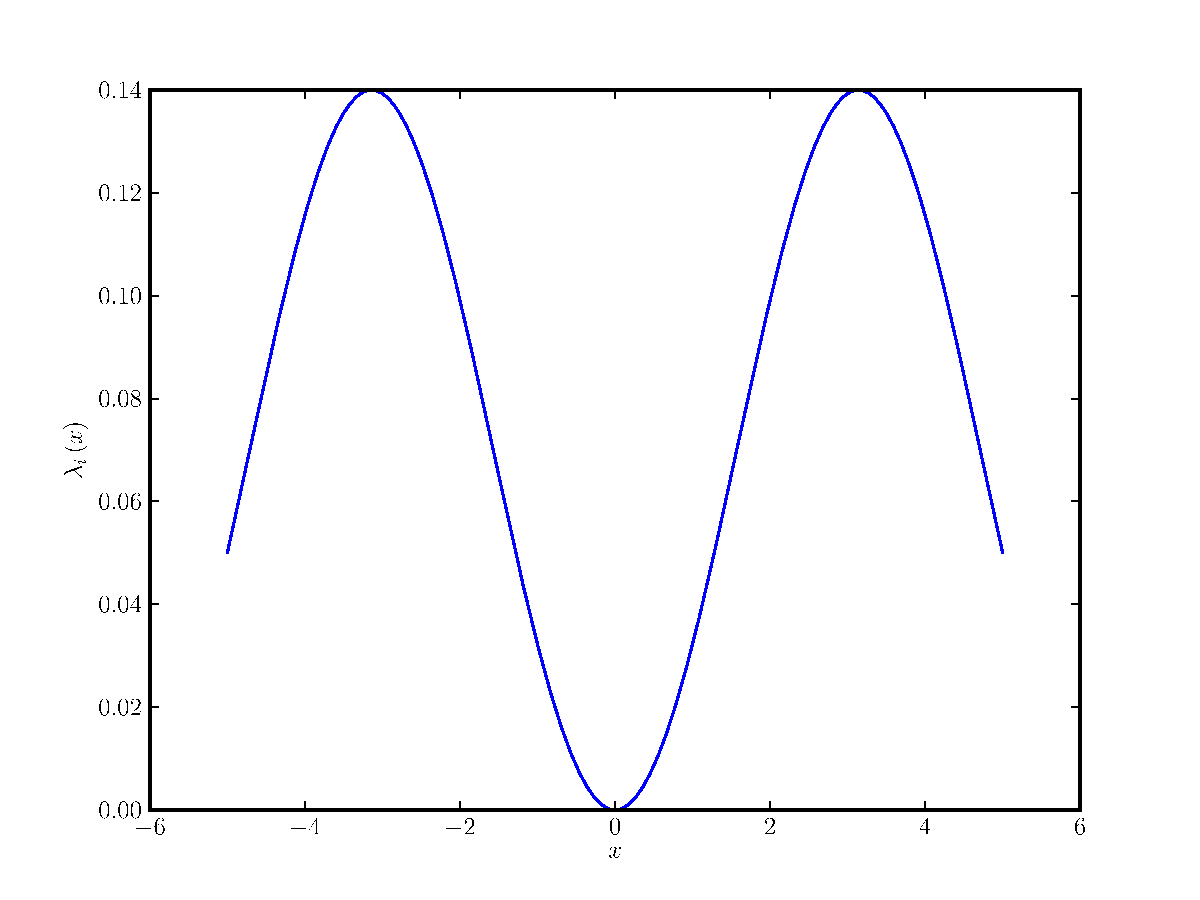
\includegraphics[scale=0.25]{./fig/cos_waves.pdf}
  \end{center}
\end{minipage}


\begin{minipage}{0.5\linewidth}
  Name:    \texttt{double\_well}
  \begin{equation*}
    V\ofs{x} = \left(\begin{smallmatrix}\sigma \left(1 - x^{2}\right)^{2}\end{smallmatrix}\right)
  \end{equation*}
  Defaults:
  \begin{align*}
    \sigma & = 1.0
  \end{align*}
\end{minipage}
\begin{minipage}{0.5\linewidth}
  \begin{center}
    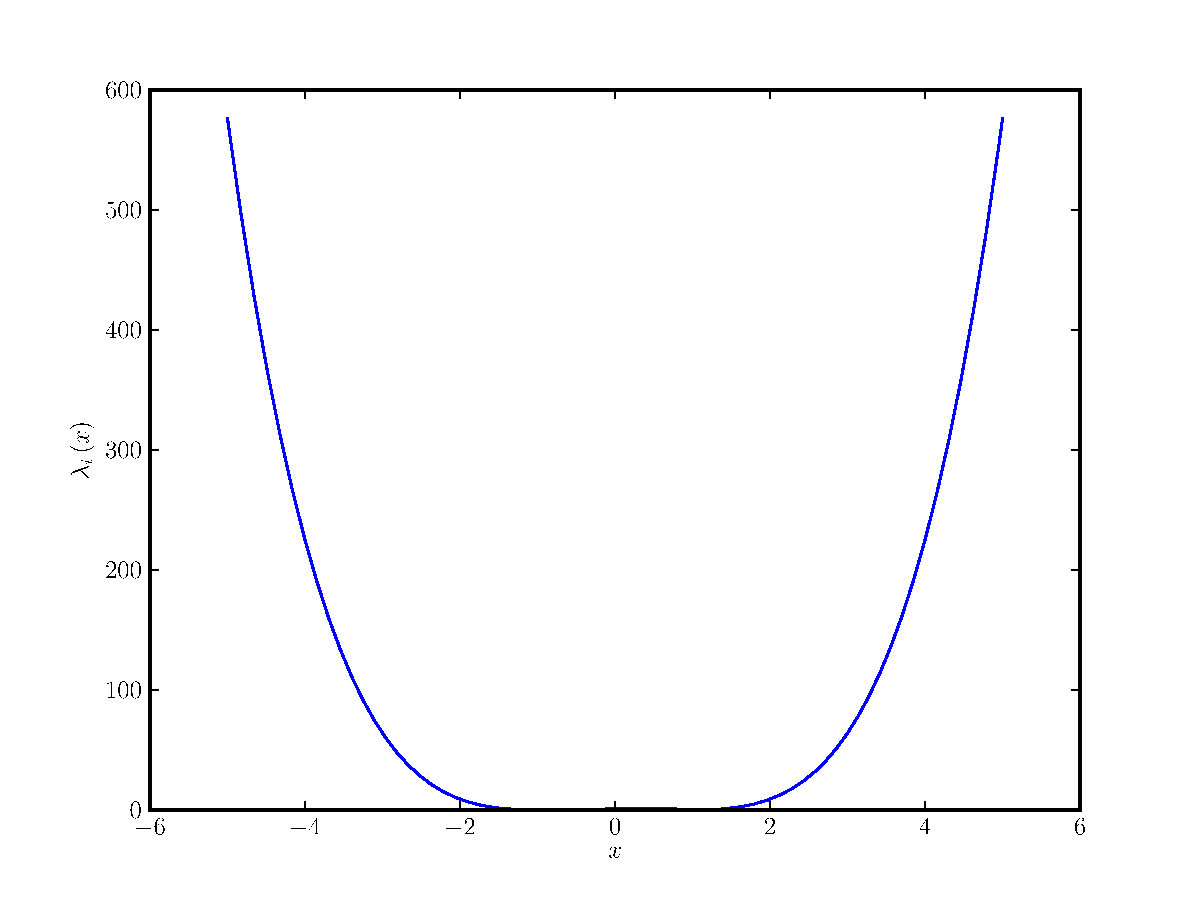
\includegraphics[scale=0.25]{./fig/double_well.pdf}
  \end{center}
\end{minipage}


\begin{minipage}{0.5\linewidth}
  Name:    \texttt{eckart}
  \begin{equation*}
    V\ofs{x} = \left(\begin{smallmatrix}\frac{\sigma}{\operatorname{cosh}^{2}\left(\frac{x}{a}\right)}\end{smallmatrix}\right)
  \end{equation*}
  Defaults:
  \begin{align*}
    \sigma & = 100 \cdot 3.8088 \cdot 10^{-4} \\
    a &= \frac{1.0}{2.0 \cdot 0.52918}
  \end{align*}
\end{minipage}
\begin{minipage}{0.5\linewidth}
  \begin{center}
    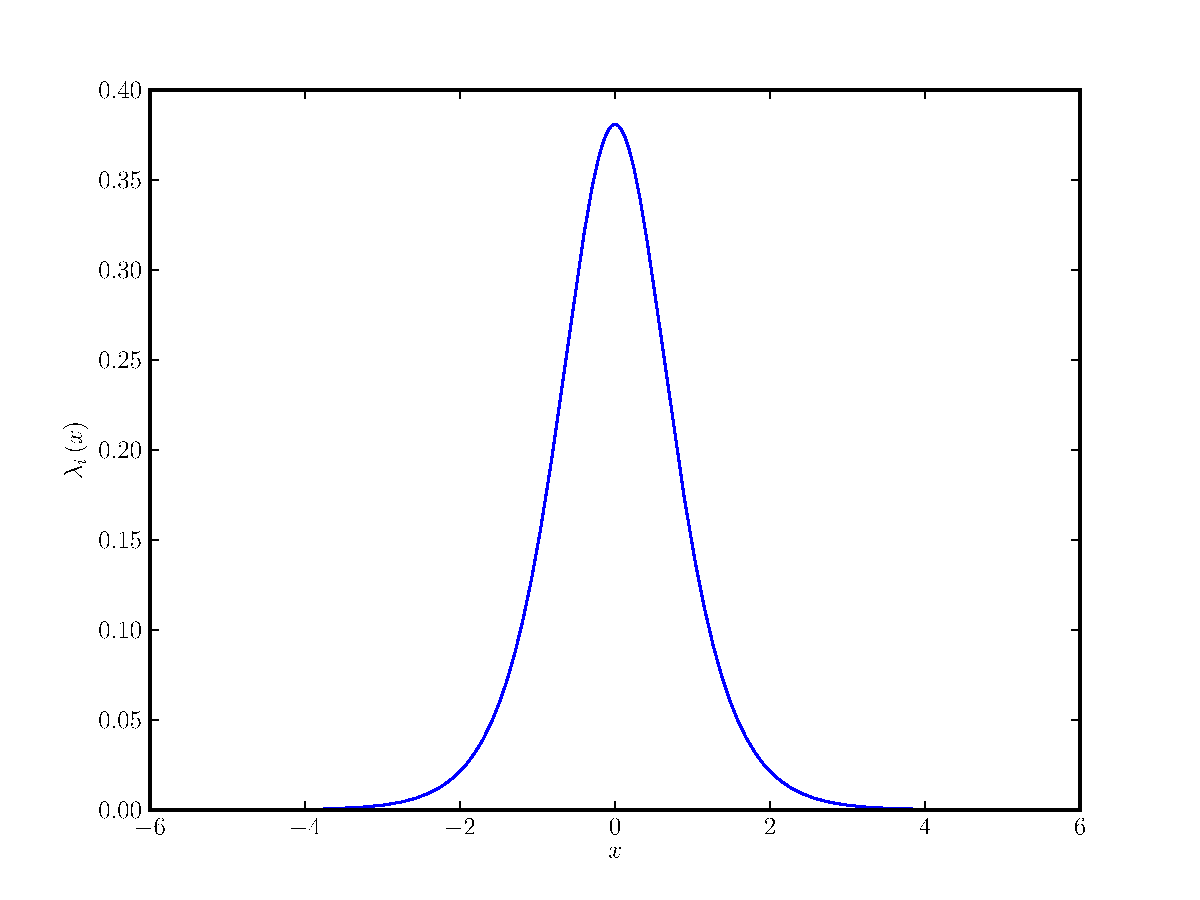
\includegraphics[scale=0.25]{./fig/eckart.pdf}
  \end{center}
\end{minipage}


\begin{minipage}{0.5\linewidth}
  Name:    \texttt{pert\_quadratic}
  \begin{equation*}
    V\ofs{x} = \left(\begin{smallmatrix}\frac{1}{2} \sigma x^{2} + \frac{1}{2} eps^{2} x^{2}\end{smallmatrix}\right)
  \end{equation*}
  Defaults:
  \begin{align*}
    \sigma & = 0.05
  \end{align*}
\end{minipage}
\begin{minipage}{0.5\linewidth}
  \begin{center}
    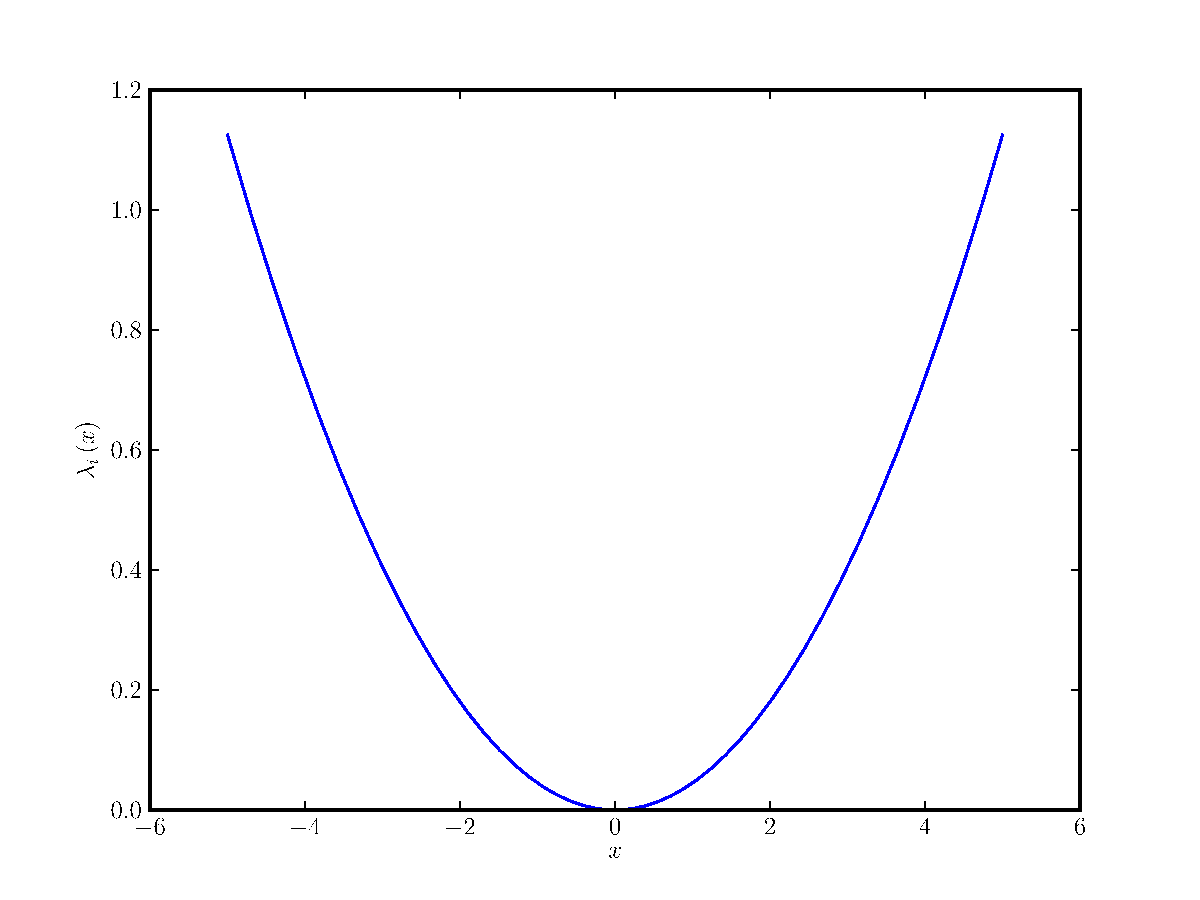
\includegraphics[scale=0.25]{./fig/pert_quadratic.pdf}
  \end{center}
\end{minipage}


\begin{minipage}{0.5\linewidth}
  Name:    \texttt{quadratic}
  \begin{equation*}
    V\ofs{x} = \left(\begin{smallmatrix}\frac{1}{2} \sigma x^{2}\end{smallmatrix}\right)
  \end{equation*}
  Defaults:
  \begin{align*}
    \sigma & = 0.5
  \end{align*}
\end{minipage}
\begin{minipage}{0.5\linewidth}
  \begin{center}
    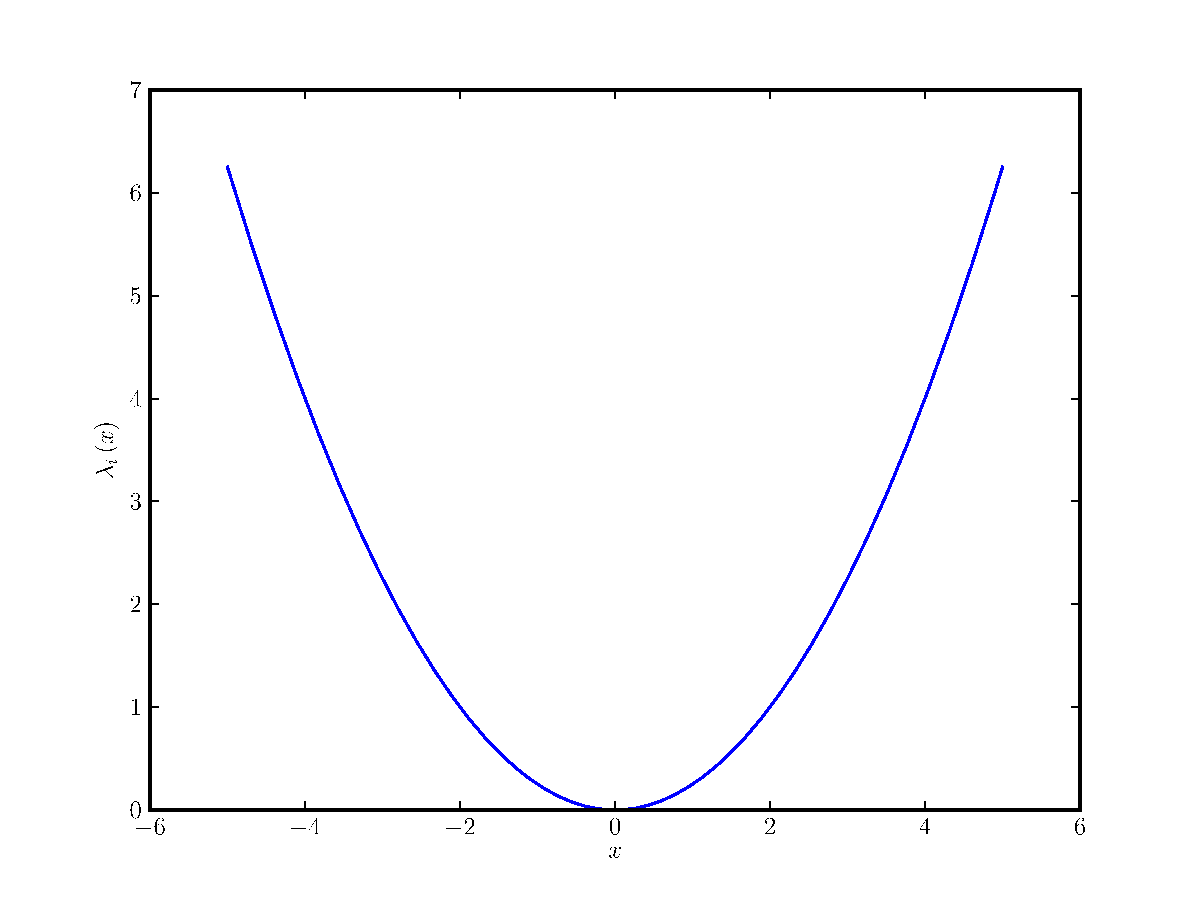
\includegraphics[scale=0.25]{./fig/quadratic.pdf}
  \end{center}
\end{minipage}


\begin{minipage}{0.5\linewidth}
  Name:    \texttt{quartic}
  \begin{equation*}
    V\ofs{x} = \left(\begin{smallmatrix}\frac{1}{4} \sigma x^{4}\end{smallmatrix}\right)
  \end{equation*}
  Defaults:
  \begin{align*}
    \sigma & = 0.05
  \end{align*}
\end{minipage}
\begin{minipage}{0.5\linewidth}
  \begin{center}
    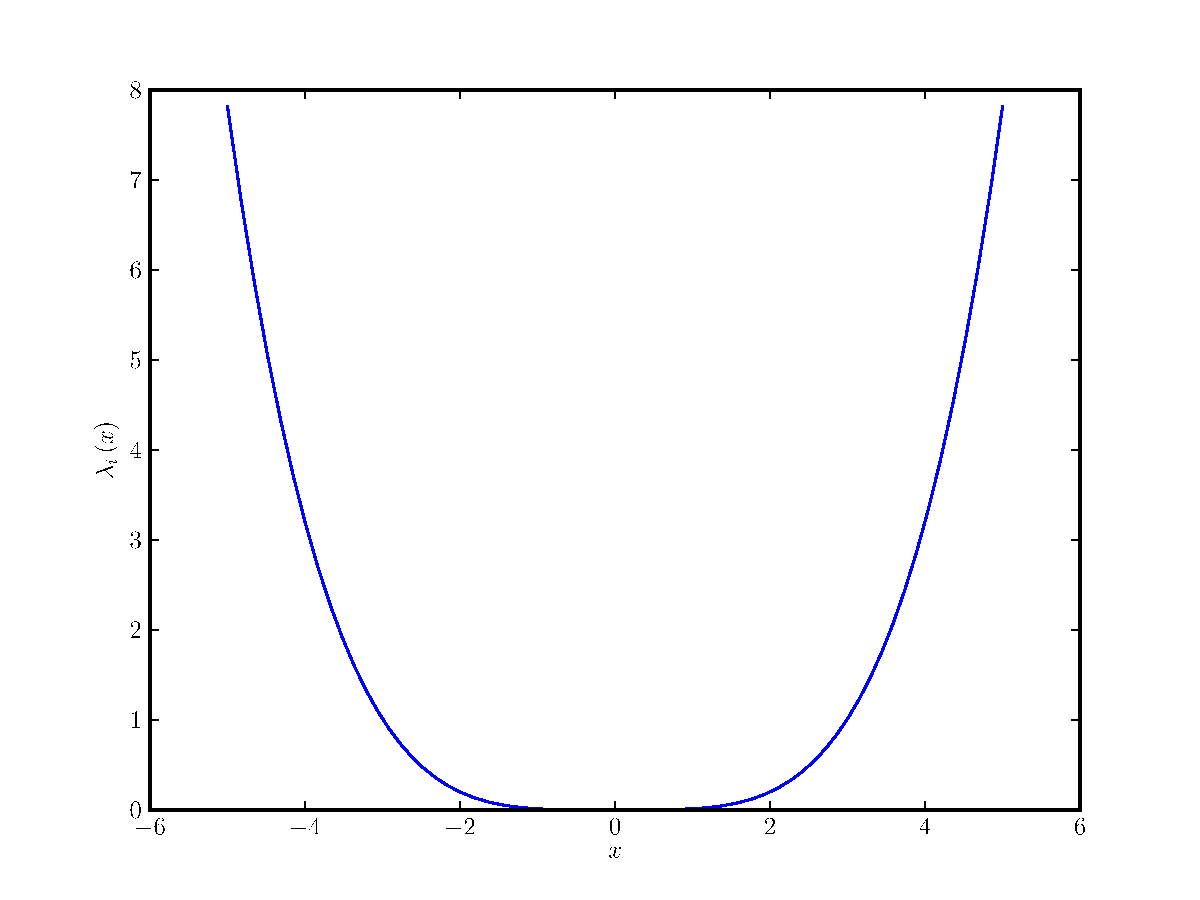
\includegraphics[scale=0.25]{./fig/quartic.pdf}
  \end{center}
\end{minipage}


\begin{minipage}{0.5\linewidth}
  Name:    \texttt{v\_shape}
  \begin{equation*}
    V\ofs{x} = \left(\begin{smallmatrix}\frac{1}{2} \sqrt{\operatorname{tanh}^{2}\left(x\right) + \frac{9}{16} eps^{2}}\end{smallmatrix}\right)
  \end{equation*}
\end{minipage}
\begin{minipage}{0.5\linewidth}
  \begin{center}
    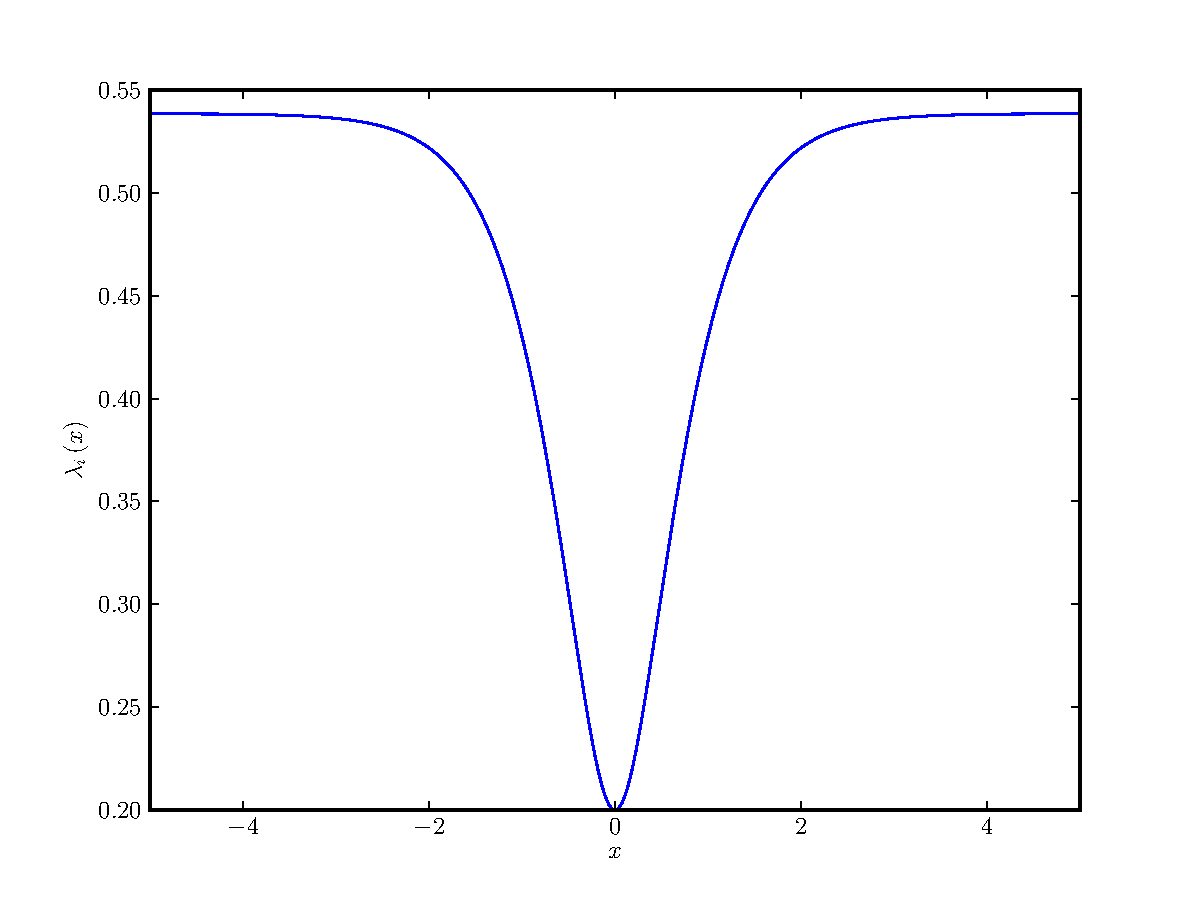
\includegraphics[scale=0.25]{./fig/v_shape.pdf}
  \end{center}
\end{minipage}


\begin{minipage}{0.5\linewidth}
  Name:    \texttt{wall}
  \begin{equation*}
    V\ofs{x} = \left(\begin{smallmatrix}\frac{1}{2} \pi + \operatorname{atan}\left(\sigma x\right)\end{smallmatrix}\right)
  \end{equation*}
  Defaults:
  \begin{align*}
    \sigma & = 10.0
  \end{align*}
\end{minipage}
\begin{minipage}{0.5\linewidth}
  \begin{center}
    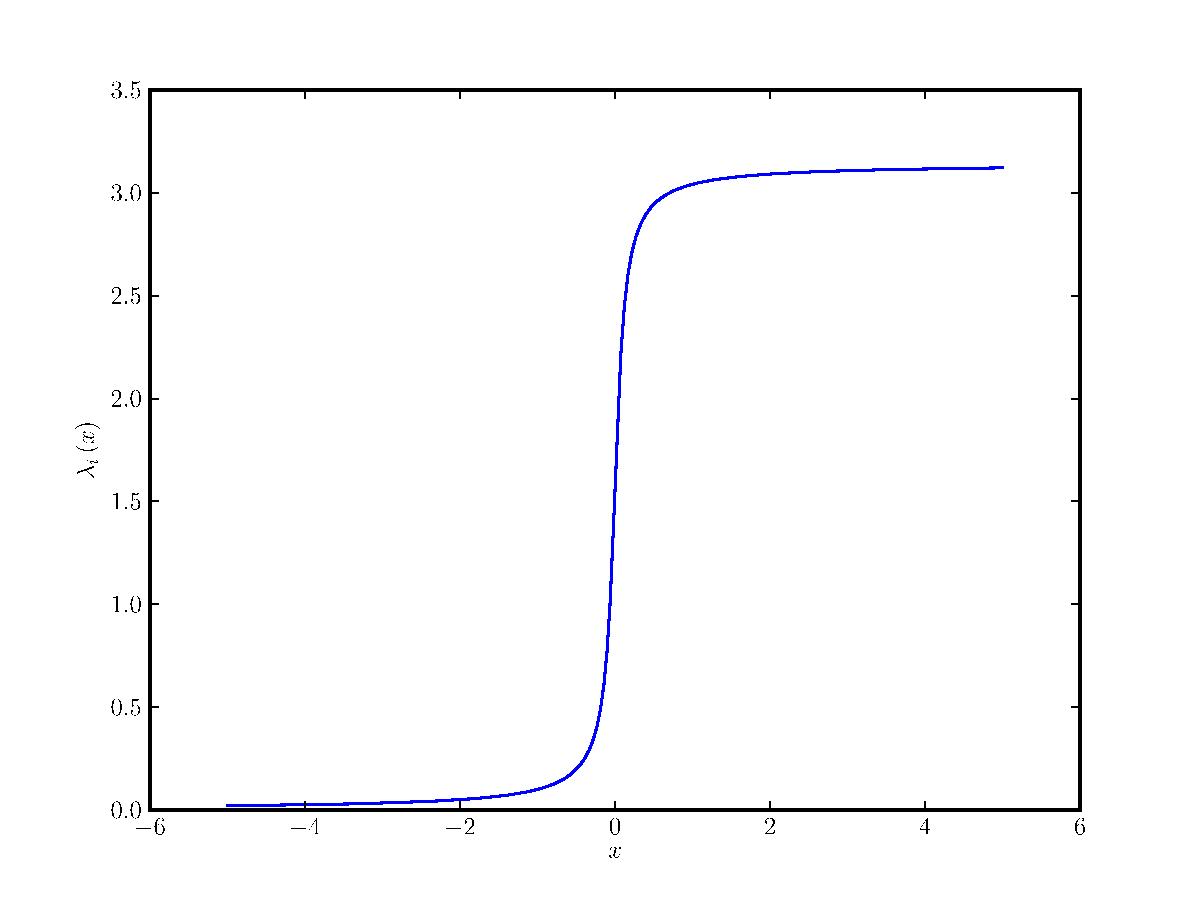
\includegraphics[scale=0.25]{./fig/wall.pdf}
  \end{center}
\end{minipage}


\subsubsection{Potentials with two energy levels}


\begin{minipage}{0.5\linewidth}
  Name:    \texttt{delta\_gap}
  \begin{equation*}
    V\ofs{x} = \left(\begin{smallmatrix}\frac{1}{2} \operatorname{tanh}\left(x\right) & \delta\\\delta & - \frac{1}{2} \operatorname{tanh}\left(x\right)\end{smallmatrix}\right)
  \end{equation*}
\end{minipage}
\begin{minipage}{0.5\linewidth}
  \begin{center}
    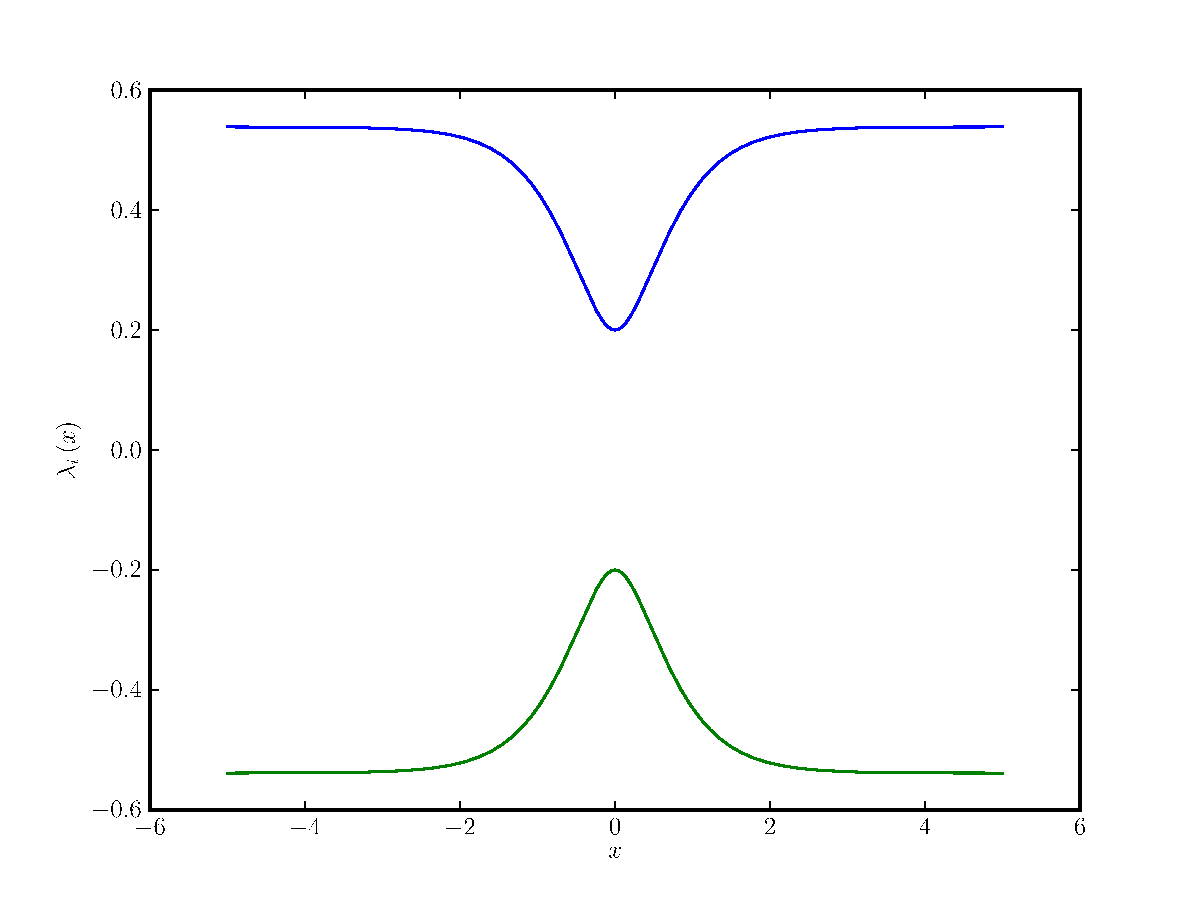
\includegraphics[scale=0.25]{./fig/delta_gap.pdf}
  \end{center}
\end{minipage}


\begin{minipage}{0.5\linewidth}
  Name:    \texttt{delta\_gap\_diag}
  \begin{equation*}
    V\ofs{x} = \left(\begin{smallmatrix}\sqrt{\delta^{2} + \frac{1}{4} \operatorname{tanh}^{2}\left(x\right)} & 0\\0 & - \sqrt{\delta^{2} + \frac{1}{4} \operatorname{tanh}^{2}\left(x\right)}\end{smallmatrix}\right)
  \end{equation*}
\end{minipage}
\begin{minipage}{0.5\linewidth}
  \begin{center}
    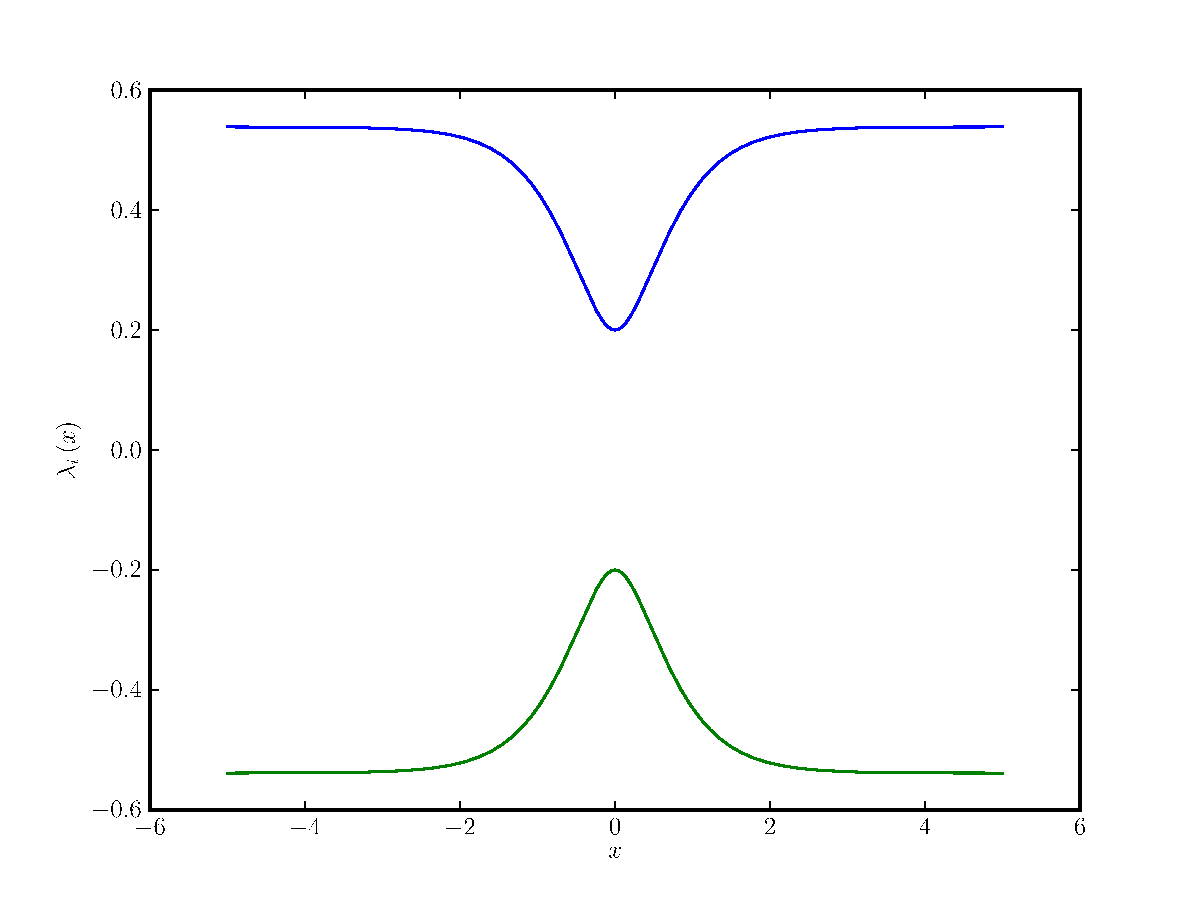
\includegraphics[scale=0.25]{./fig/delta_gap_diag.pdf}
  \end{center}
\end{minipage}


\begin{minipage}{0.75\linewidth}
  Name:    \texttt{two\_crossings}
  \begin{equation*}
    V\ofs{x} = \left(\begin{smallmatrix}\operatorname{tanh}\left(\rho + x\right) \operatorname{tanh}\left(x - \rho\right) & \delta\\\delta & - \operatorname{tanh}\left(\rho + x\right) \operatorname{tanh}\left(x - \rho\right)\end{smallmatrix}\right)
  \end{equation*}
  Defaults:
  \begin{align*}
    \rho & = 3.0
  \end{align*}
\end{minipage}
\begin{minipage}{0.25\linewidth}
  \begin{center}
    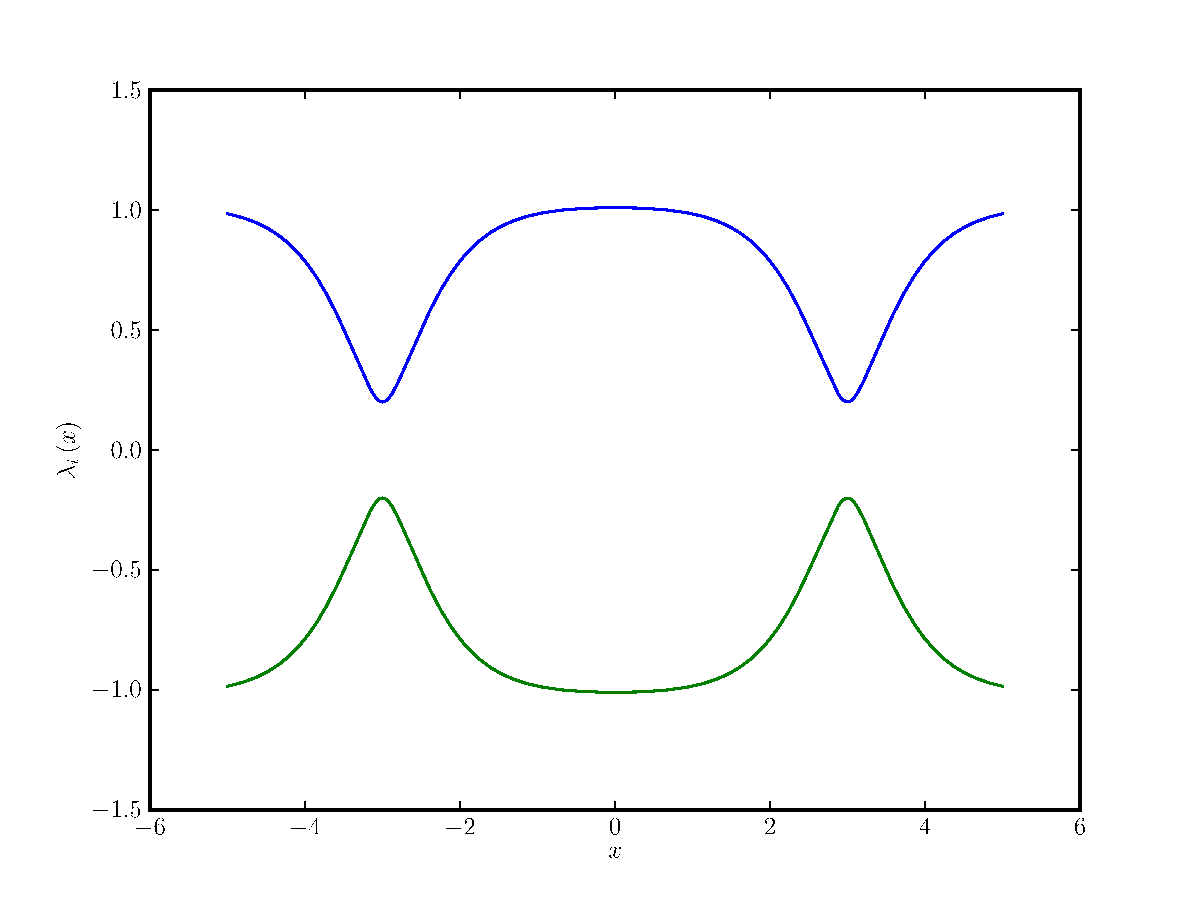
\includegraphics[scale=0.25]{./fig/two_crossings.pdf}
  \end{center}
\end{minipage}


\begin{minipage}{0.5\linewidth}
  Name:    \texttt{two\_quadratic}
  \begin{equation*}
    V\ofs{x} = \left(\begin{smallmatrix}\frac{1}{2} \sigma x^{2} & 0\\0 & \frac{1}{2} \sigma x^{2}\end{smallmatrix}\right)
  \end{equation*}
  Defaults:
  \begin{align*}
    \sigma & = 0.05
  \end{align*}
\end{minipage}
\begin{minipage}{0.5\linewidth}
  \begin{center}
    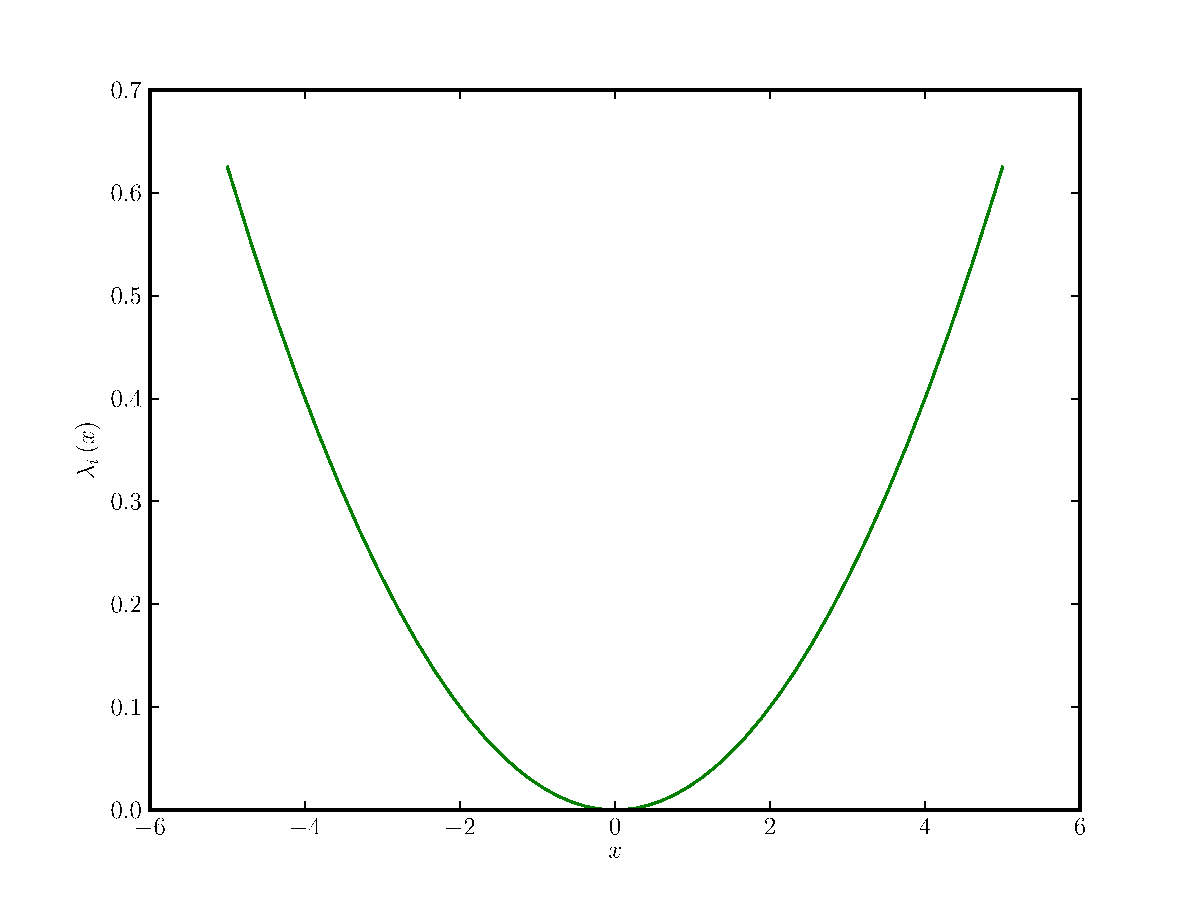
\includegraphics[scale=0.25]{./fig/two_quadratic.pdf}
  \end{center}
\end{minipage}


\begin{minipage}{0.5\linewidth}
  Name:    \texttt{two\_quartic}
  \begin{equation*}
    V\ofs{x} = \left(\begin{smallmatrix}\frac{1}{4} \sigma x^{4} & 0\\0 & \frac{1}{8} \sigma x^{4}\end{smallmatrix}\right)
  \end{equation*}
  Defaults:
  \begin{align*}
    \sigma & = 1.0
  \end{align*}
\end{minipage}
\begin{minipage}{0.5\linewidth}
  \begin{center}
    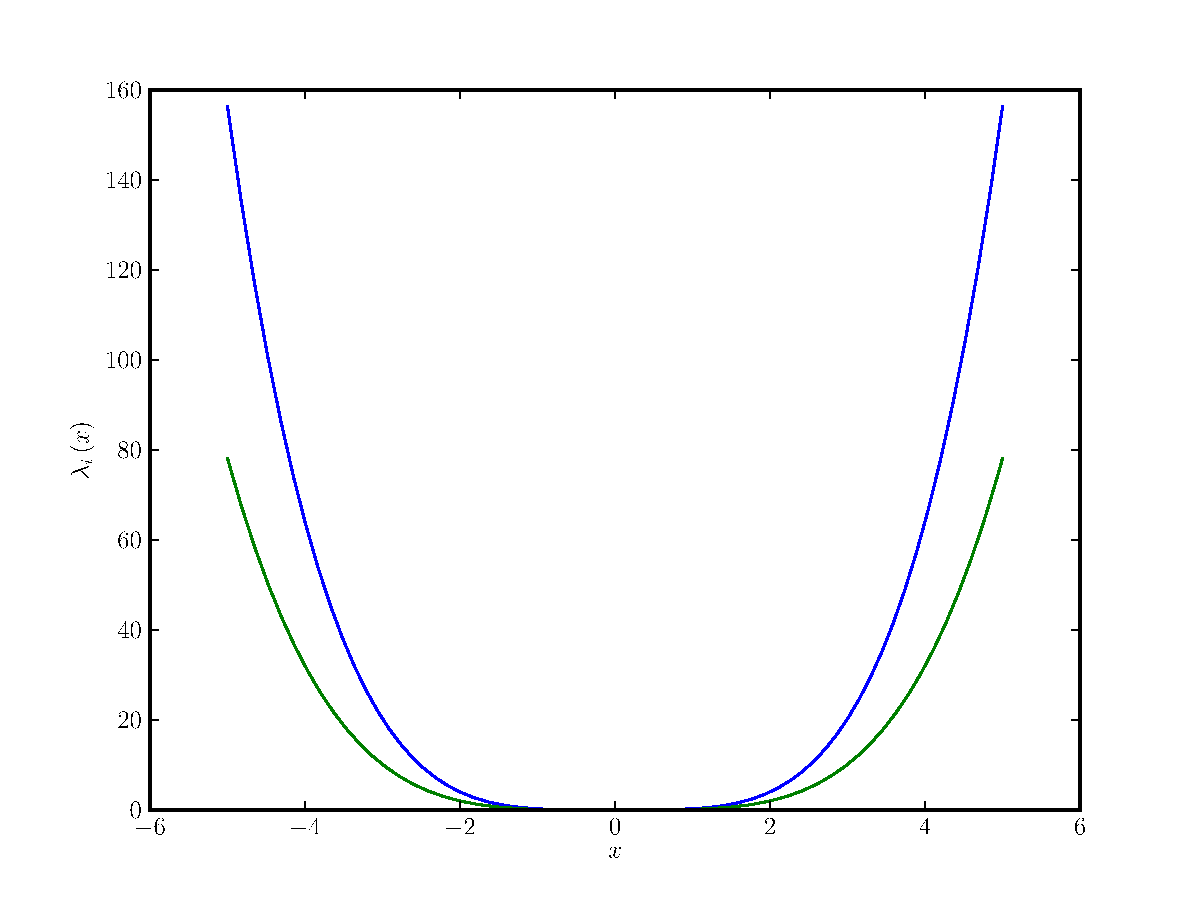
\includegraphics[scale=0.25]{./fig/two_quartic.pdf}
  \end{center}
\end{minipage}


\subsubsection{Potentials with three energy levels}


\begin{minipage}{0.75\linewidth}
  Name:    \texttt{three\_levels}
  \begin{equation*}
    V\ofs{x} = \left(\begin{smallmatrix}\operatorname{tanh}\left(\rho + x\right) + \operatorname{tanh}\left(x - \rho\right) & \delta_{1} & \delta_{2}\\\delta_{1} & - \operatorname{tanh}\left(\rho + x\right) & 0\\\delta_{2} & 0 & 1 - \operatorname{tanh}\left(x - \rho\right)\end{smallmatrix}\right)
  \end{equation*}
  Defaults:
  \begin{align*}
    \rho & = 3.0
  \end{align*}
\end{minipage}
\begin{minipage}{0.25\linewidth}
  \begin{center}
    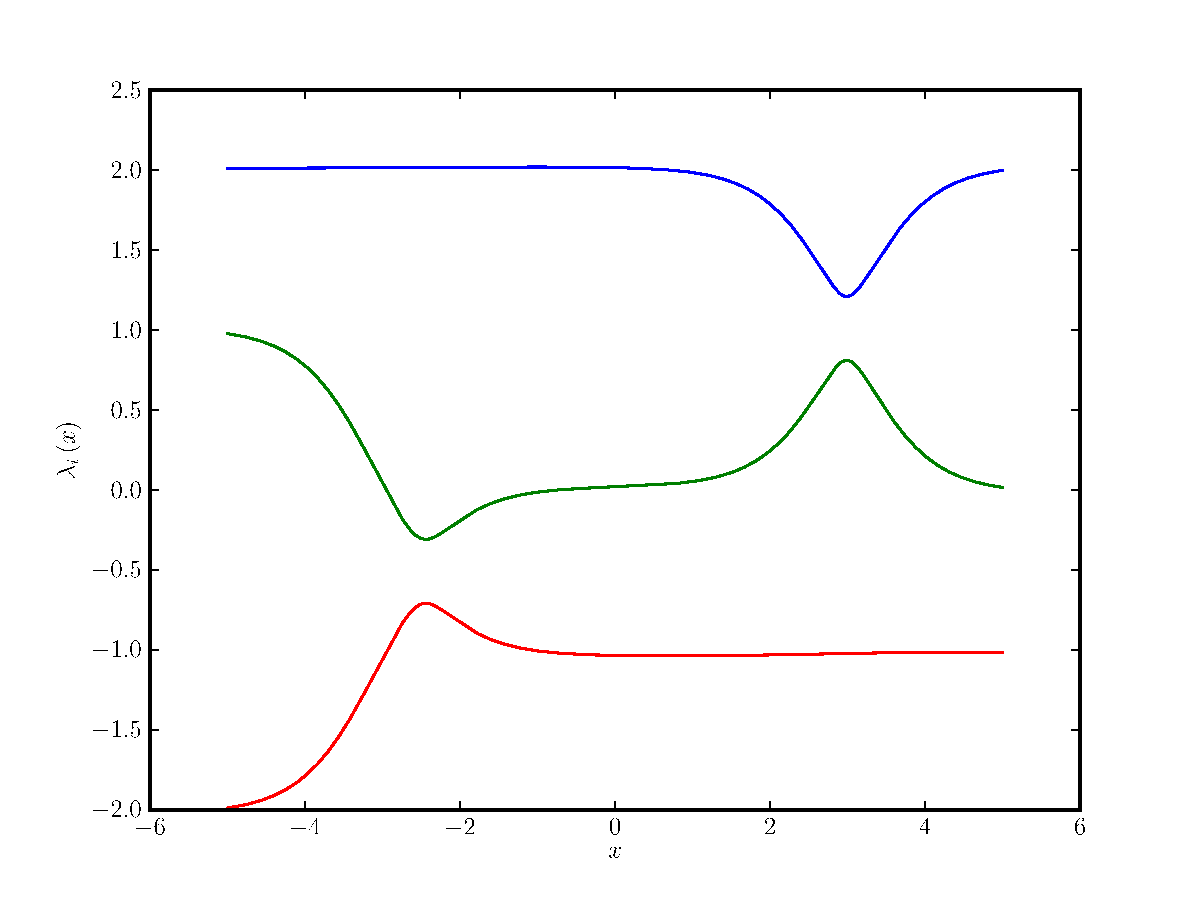
\includegraphics[scale=0.25]{./fig/three_levels.pdf}
  \end{center}
\end{minipage}


\begin{minipage}{0.5\linewidth}
  Name:    \texttt{three\_quadratic}
  \begin{equation*}
    V\ofs{x} = \left(\begin{smallmatrix}\frac{1}{2} \sigma x^{2} & 0 & 0\\0 & \frac{1}{2} \sigma x^{2} & 0\\0 & 0 & \frac{1}{2} \sigma x^{2}\end{smallmatrix}\right)
  \end{equation*}
  Defaults:
  \begin{align*}
    \sigma & = 0.05
  \end{align*}
\end{minipage}
\begin{minipage}{0.5\linewidth}
  \begin{center}
    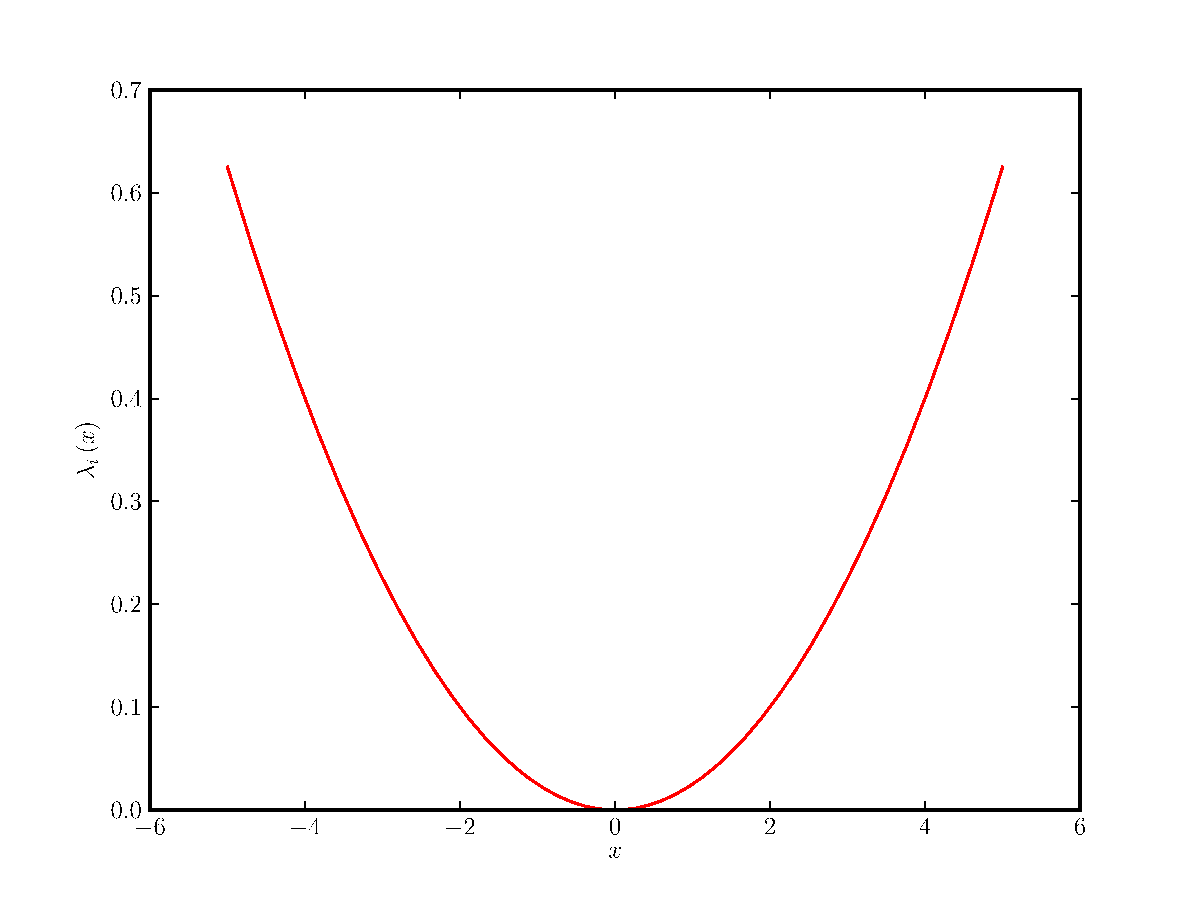
\includegraphics[scale=0.25]{./fig/three_quadratic.pdf}
  \end{center}
\end{minipage}


\subsubsection{Potentials with four energy levels}


\begin{minipage}{0.5\linewidth}
  Name:    \texttt{four\_powers}
  \begin{equation*}
    V\ofs{x} = \left(\begin{smallmatrix}\frac{1}{2} \sigma x^{2} & 0 & 0 & 0\\0 & \frac{1}{4} \sigma x^{4} & 0 & 0\\0 & 0 & \frac{1}{6} \sigma x^{6} & 0\\0 & 0 & 0 & \frac{1}{8} \sigma x^{8}\end{smallmatrix}\right)
  \end{equation*}
  Defaults:
  \begin{align*}
    \sigma & = 0.05
  \end{align*}
\end{minipage}
\begin{minipage}{0.5\linewidth}
  \begin{center}
    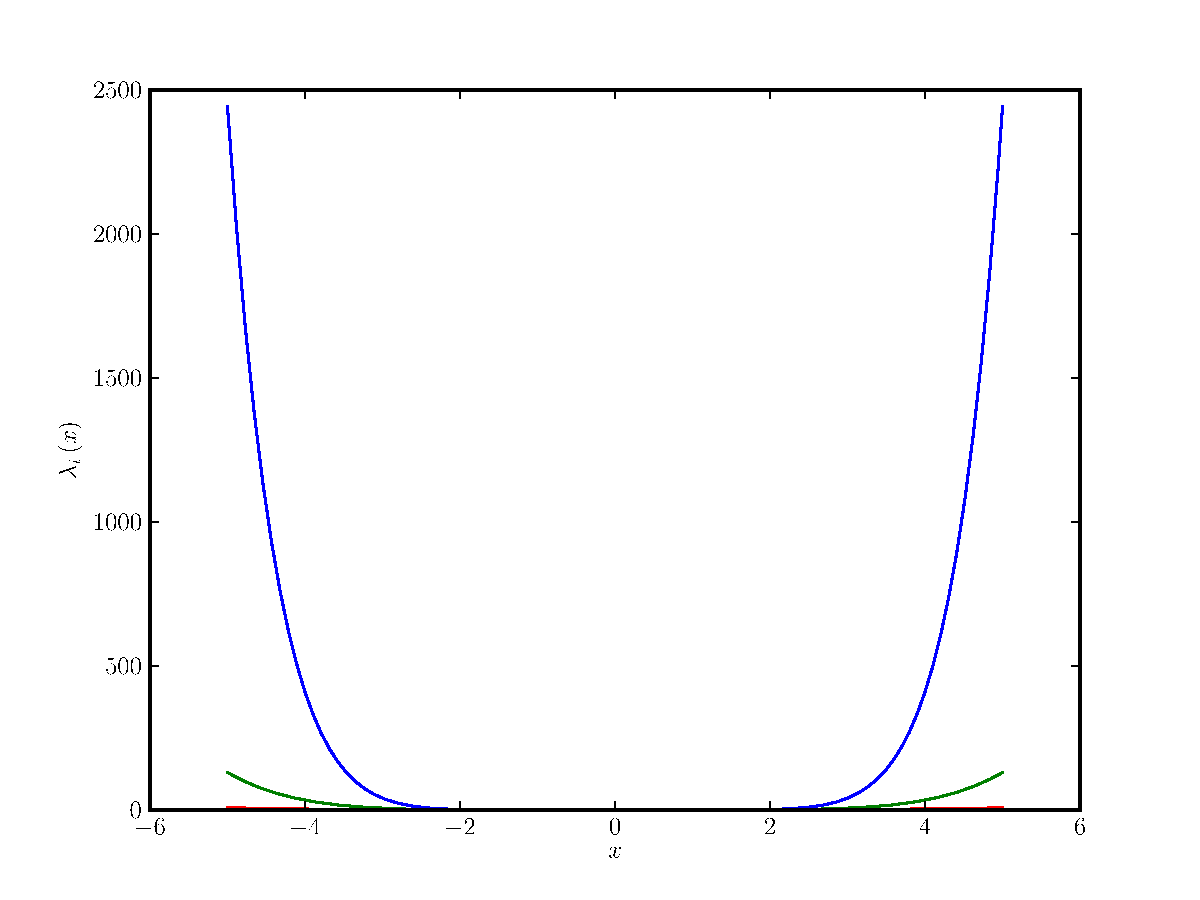
\includegraphics[scale=0.25]{./fig/four_powers.pdf}
  \end{center}
\end{minipage}


\subsubsection{Potentials with five energy levels}


\begin{minipage}{0.5\linewidth}
  Name:    \texttt{five\_quadratic}
  \begin{equation*}
    V\ofs{x} = \left(\begin{smallmatrix}\frac{1}{2} \sigma x^{2} & 0 & 0 & 0 & 0\\0 & \frac{1}{2} \sigma x^{2} & 0 & 0 & 0\\0 & 0 & \frac{1}{2} \sigma x^{2} & 0 & 0\\0 & 0 & 0 & \frac{1}{2} \sigma x^{2} & 0\\0 & 0 & 0 & 0 & \frac{1}{2} \sigma x^{2}\end{smallmatrix}\right)
  \end{equation*}
  Defaults:
  \begin{align*}
    \sigma & = 0.05
  \end{align*}
\end{minipage}
\begin{minipage}{0.5\linewidth}
  \begin{center}
    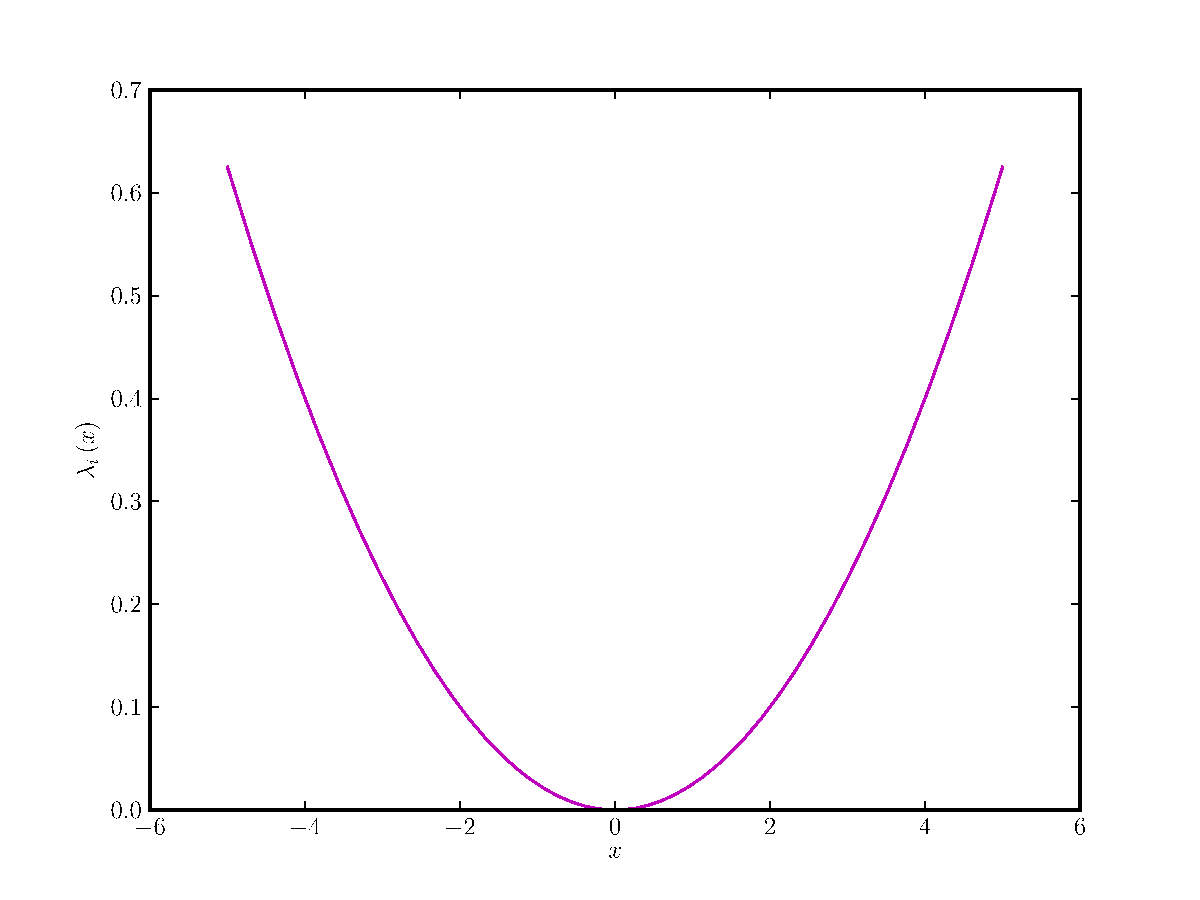
\includegraphics[scale=0.25]{./fig/five_quadratic.pdf}
  \end{center}
\end{minipage}


\subsection{Time propagation algorithms}

At the moment, three algorithms for time propagation of initial values are
implemented.

\begin{center}
\begin{tabular}{ll}
  Name & Description \\
  \hline
  \texttt{fourier} & Fourier propagation / Operator splitting \\
  \texttt{hagedorn} & Homogeneous Hagedorn wavepackets \\
  \texttt{multihagedorn} & Inhomogeneous Hagedorn wavepackets \\
%   \texttt{spawn} & Spawning propagation for tunneling problems
\end{tabular}
\end{center}


\subsection{Specifying initial values}


Initial values are always specified as wavepackets. For the Fourier propagator,
the packets are samples at the grid nodes and for packet based algorithms, these
initial packets are propagated. The two configuration variables \texttt{parameters}
and \texttt{coefficients} are responsible for specifying the initial wavepackets.
Their values are interpreted as usual.

\subsection{Required parameter sets}

The simulations can be configured with a very flexible scheme. Namely is possible
to just specify the values that are really necessary and omit all others. There
are some input parameters that have to be provided in any case and many others that
are only necessary for a specific algorithm or are pure optional.

In this section of the manual all parameters that can be provided are listed.
But you are free to define additional parameters and use them in a data evaluation
script. Just make sure there is no variable name clash.

% \begin{description}
%   \item[\texttt{}]
%   \begin{itemize}
%     \item
%     \item
%   \end{itemize}
% \end{description}

\subsubsection{Parameters for all propagation algorithms}

\begin{description}
  \item[\texttt{algorithm}] The simulation algorithm
  \begin{itemize}
    \item Possible values: \texttt{fourier}, \texttt{hagedorn}, \texttt{multihagedorn}, \texttt{spawn}
    \item Data type: string
  \end{itemize}

  \item[\texttt{potential}] The potential
  \begin{itemize}
    \item Possible values: see section \ref{sec:ready_made_potentials}
    \item Data type: string or dict
  \end{itemize}

  \item[\texttt{T}] The time when the simulation stops
  \begin{itemize}
    \item Possible values: Non-negative float
    \item Data type: float
  \end{itemize}

  \item[\texttt{dt}] The size of a single time step
  \begin{itemize}
    \item Possible values: Non-negative float
    \item Data type: float
  \end{itemize}

  \item[\texttt{eps}] The semi-classical scaling parameter
  \begin{itemize}
    \item Possible values: Non-negative float
    \item Data type: float
  \end{itemize}

  \item[\texttt{parameters}] The Hagedorn parameters $\{P, Q, S, p, q \}$ of the
    initial wave packets. The exact format of this variable depends on the
    simulation algorithm used.

  \item[\texttt{coefficients}] A list with the lists of (index,value) tuples that
    set the coefficients of the basis functions for the initial wavepackets. The
    exact format of this variable depends on the simulation algorithm used.

  \item[\texttt{write\_nth}] Save simulation data every n-th timestep
  \begin{itemize}
    \item Possible values: Positive Integer where the case 0 is interpreted as
          \emph{never}. In this case only the initial values are saved.
    \item Data type: integer
    \item Default value: is 0 if no other value is provided.
  \end{itemize}

  \item[\texttt{save\_at}] A list of times and/or timesteps when saving of the
    simulation data takes place. (Which data are saved depends on the implementation
    of the respective \texttt{SimulationLoop} subclass.)
  \begin{itemize}
    \item Possible values: A list of integers and/or floats. Integers are interpreted
    as timesteps and floats as (absolute) times. Be always aware of this difference
    in interpretation!
    \item Data type: integer or float
    \item Default value: an empty list, thus saving at special points in time
    is not enabled.
  \end{itemize}
\end{description}

\subsubsection{Parameters for the \texttt{fourier} propagator}

\begin{description}
  \item[\texttt{ngn}] The number of grid nodes used for the Fourier transformation.
  \begin{itemize}
    \item Possible values: Integer, optimal is a power of 2 but this is not necessary.
    \item Data type: integer
  \end{itemize}

  \item[\texttt{f}] A scalar number that determines the extension of the computational domain.
  \begin{itemize}
    \item Possible values: A non-negative float
    \item Data type: float
  \end{itemize}
\end{description}

\subsubsection{Parameters for the \texttt{hagedorn} propagator}

\begin{description}
  \item[\texttt{basis\_size}] Number of basis functions used for homogeneous Hagedorn wavepackets.
  \begin{itemize}
    \item Possible values: Non-negative integer larger than $2$.
    \item Data type: integer
  \end{itemize}

  \item[\texttt{leading\_component}] The leading component is the eigenvalue that
    governs the propagation of the wavepackets' parameters.
  \begin{itemize}
    \item Possible values: Integer in the range $0$ to $N-1$ inclusive, where $N$
      is the number of energy levels the given potential supports.
    \item Data type: integer
  \end{itemize}
\end{description}

\subsubsection{Parameters for the \texttt{multihagedorn} propagator}

\begin{description}
  \item[\texttt{basis\_size}] Number of basis functions used for inhomogeneous hagedorn packets.
  \begin{itemize}
    \item Possible values: Non-negative integer larger than $2$.
    \item Data type: integer
  \end{itemize}
\end{description}

% \subsubsection{Parameters for the \texttt{spawn} propagator}
%
% \begin{description}
%   \item[\texttt{K0}] The index of the coefficient where splitting is applied.
%   \begin{itemize}
%     \item Non-negative integer in the range $\left[0, \ldots, K\right]$ where $K$
%           is the basis size.
%   \end{itemize}
%
%   \item[\texttt{threshold}] The spawning threshold that determined when to spawn.
%   \begin{itemize}
%     \item Non-negative float.
%   \end{itemize}
% \end{description}

\subsubsection{Optional parameters}

All variables that appear as parameters of some potential can be specified
here. For example, the \texttt{quadratic} potential has a parameter \texttt{sigma}
which can be given in the simulation configuration. (Otherwise a default value
would be used.) For potentials that contain parameters for which no default
values are specified, these parameters must be given in the configuration file.
An example of such a parameter is the \texttt{delta} of the \texttt{delta\_gap} potential.


\section{Data storage}

What data get written to disk. How can we retrieve data, IOM basics, usage, etc

\subsection{How IOM works}

\subsection{What gets stored}

\subsubsection{Retrieving the simulation parameters}

From a hdf5 file with the simulation data we can get back the parameters this
simulation used. Retrieval is trivial, the following commented interactive python
session shows the basics which can of course be used in a user script too.

\begin{verbatim}
  >>> from WaveBlocks import IOManager
  >>> iom = IOManager()                         # create an IOM instance
  >>> iom.load_file("simulation_results.hdf5")  # load the data file
  >>> sim_params = iom.get_parameters()         # request the parameters
  >>> print(sim_params)
  ====================================
  Parameters of the current simulation
  ------------------------------------
  [...]
\end{verbatim}

\subsubsection{Load simulation data}

How to get particular simulation data


\section{User scripts}

Consider merging this section with chaper 2.
Do an explicit example walk through somewhere.

\subsection{Preparing simulations}

\begin{verbatim}
  python ConfigurationGenerator.py  <metaconfiguration.py> <configurations_dir>
\end{verbatim}


\subsection{Generating Configurations}

In detail description on how to generate valid configurations

\subsubsection{Manually}

\subsubsection{Meta-configurations}

\begin{verbatim}
- You can use any valid python statement as value
- All statements are written to a pure python code file
- You can write numbers, lists etc as plain text strings
- All that is not in string form gets evaluated *right now*
- Remember to escape python strings twice
- You can use variable references but with great care!
- The ordering of the statements in the output file is such that
  all statements can be executed w.r.t. local variables. This is
  some kind of topological sorting. Be warned, it's implemented
  using black magic and may fail now and then!

  That should be all ...
\end{verbatim}

\subsection{Running simulations}

\begin{verbatim}
  python Main.py <simulationparameters.py>
\end{verbatim}

\begin{verbatim}
  python Batch.py <batchconfiguration.py> <configurations_dir> <results_dir>
\end{verbatim}





\subsection{Computing additional data}

Only compute/store what comes out directly from the time propagation
(Or what would be much more difficult to computer afterwards)

Compute all other data in a separate step after the simulation finished
Example: Norms, energies etc

\subsection{Evaluating data}

\subsection{Plot data}

Call plot scripts which load the simulation data from a file and plot the values.



\chapter{The \texttt{WaveBlocks} library}

\section{Available blocks}

See the API documentation.

\chapter{Extending the \texttt{WaveBlocks} Core}

In this chapter we describe what it takes to extend the \texttt{WaveBlocks}
code base with respect to various central aspects.

\section{New potentials}

Adding new potentials to the potential library.
A word about parameters used for the potentials.

\section{Compute and store more data}

IOM and IOM Plugins, how to teach the IOM to store more/other data.

\section{New propagation algorithms}

Implementing the \texttt{SimulationLoop} and \texttt{Propagator} interfaces



\chapter{For developers, Software architecture}

\section{Interfaces}

\section{Class hierarchies}

\end{document}
